\documentclass[12pt,a4paper,oneside]{report}

\usepackage[margin=1in,headheight=15pt]{geometry}
\usepackage{pdfpages}
\usepackage{graphicx}
\usepackage{float}
\usepackage{booktabs}
\usepackage{longtable}
\usepackage{array}
\usepackage{multirow}
\usepackage{amsmath,amssymb}
\usepackage{siunitx}
\usepackage{xcolor}
\usepackage{caption}
\usepackage{subcaption}
\usepackage{enumitem}
\usepackage{setspace}
\usepackage{fancyhdr}
\usepackage{hyperref}
\usepackage{microtype}
\usepackage{tikz}
\usetikzlibrary{arrows.meta,positioning,shapes.geometric}

\definecolor{IITNavy}{HTML}{173B5E}
\definecolor{IITGold}{HTML}{B88936}
\definecolor{SoftBlue}{HTML}{EAF3F7}
\definecolor{SoftRed}{HTML}{F7ECEE}
\definecolor{Muted}{HTML}{596B78}
\hypersetup{
  colorlinks=true,
  linkcolor=IITNavy,
  citecolor=IITNavy,
  urlcolor=IITNavy,
  pdftitle={Prediction of Properties of Additively Manufactured Parts for Haynes 282: Experimental Validation and Joint Inverse Design},
  pdfauthor={Taha Hassan Khan; Shivarpan Tyagi; Shivam Kumar; Prachi Singh; Satyam Kumar Mishra}
}
\setstretch{1.12}
\setlength{\parskip}{0.25em}
\setlength{\parindent}{1.5em}
\setlist[itemize]{itemsep=0.25em,topsep=0.35em}
\setlist[enumerate]{itemsep=0.3em,topsep=0.35em}
\captionsetup{font=small,labelfont=bf}
\sisetup{detect-all,group-separator={,}}
\graphicspath{{figures/}}

\pagestyle{fancy}
\fancyhf{}
\fancyfoot[C]{\thepage}
\renewcommand{\headrulewidth}{0pt}
\renewcommand{\footrulewidth}{0pt}

\newcommand{\placeholder}[2]{%
  \begin{center}
  \fbox{\begin{minipage}[c][#1][c]{0.88\textwidth}\centering\color{Muted}\Large #2\end{minipage}}
  \end{center}}
\newcommand{\Rtwo}{\ensuremath{R^2}}
\newcommand{\VED}{\ensuremath{E_{\mathrm{vol}}}}
\newcommand{\HV}{\ensuremath{\mathrm{HV}}}

\begin{document}

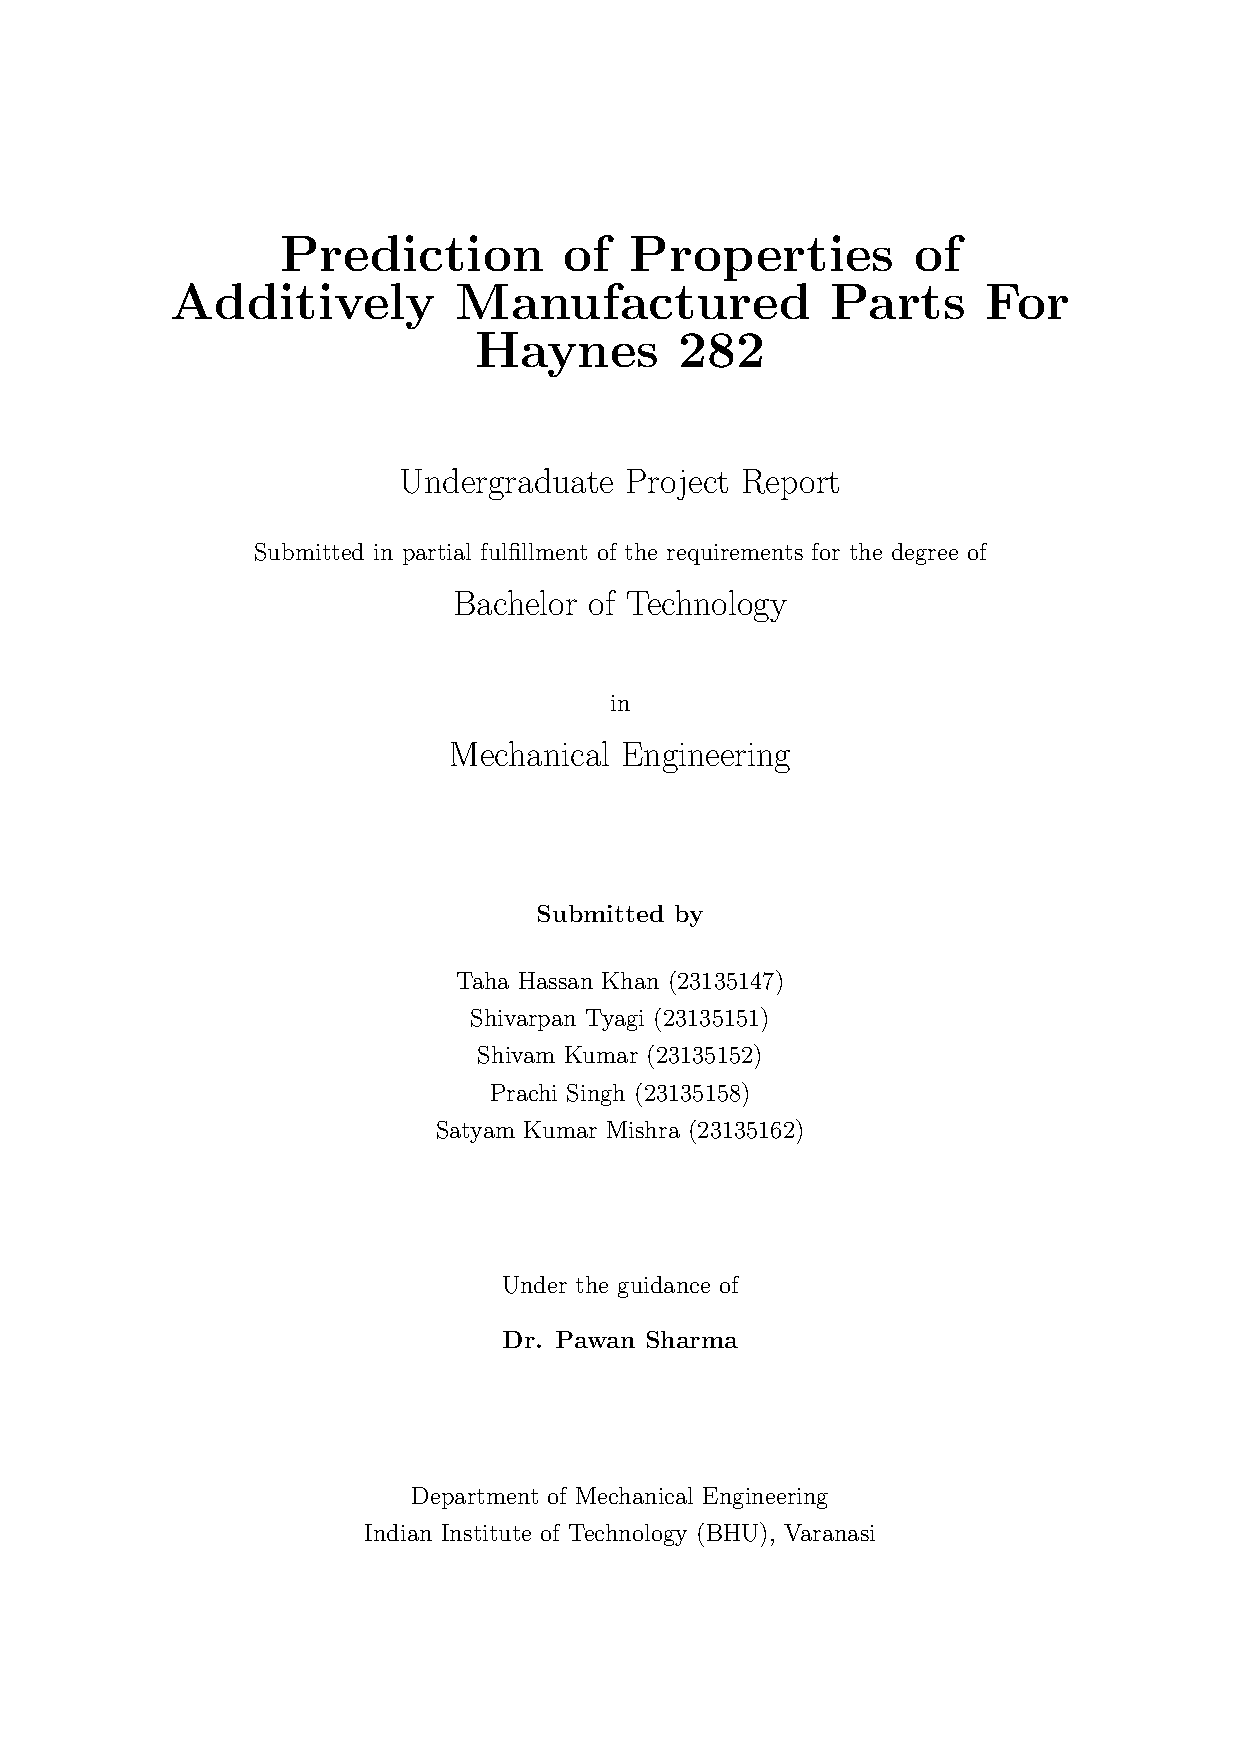
\includepdf[pages=1-3]{front_matter.pdf}
\setcounter{chapter}{2}
\addtocontents{toc}{\protect\contentsline{chapter}{\protect\numberline{1}Introduction}{5}{}}
\addtocontents{toc}{\protect\contentsline{chapter}{\protect\numberline{2}Literature Review}{8}{}}
\tableofcontents
\clearpage

% The imported Part I chapters follow the contents page.
\includepdf[pages=4-10]{front_matter.pdf}
\setcounter{page}{13}

\chapter{Updated Methodology and Validation Design}

\section{Purpose of the continuation}
The first part of the project established a data-driven workflow for LPBF property prediction and process-parameter search for Haynes 282. The present continuation concentrates on the experimental mechanical-property measurements and on a more explicit evaluation design for hardness, ultimate tensile strength (UTS), and relative density. The central objective is not to claim that synthetic augmentation creates new physical evidence. Instead, it is to use the available measurements efficiently, quantify uncertainty and prediction error at known settings, and use the forward models to shortlist process conditions for future builds.

The current mechanical-property table contains paired UTS and density measurements for the same sample identifiers used in the hardness workbook. Hardness readings were recorded in two orientations and combined using the arithmetic mean of the orientation means. This gives perpendicular and parallel orientations equal weight even though the number of indent readings differs. The resulting composite target is expressed in HV; the earlier report's HRA values are not mixed into this analysis.

\section{Inputs, outputs, and derived process quantity}
The model inputs are laser power $P$ in watts, scan speed $v$ in millimetres per second, hatch distance $h$ in millimetres, and layer thickness $t$ in millimetres. Layer thickness is fixed at \SI{0.04}{mm} in the current measured campaign. The model outputs used by the joint inverse workflow are hardness in HV, UTS in MPa, and relative density in percent. The volumetric energy density is calculated as
\begin{equation}
  \VED = \frac{P}{v h t},
  \label{eq:ved}
\end{equation}
with units of \si{J.mm^{-3}} when the inputs are expressed in the units above. It is used as a process-window constraint and diagnostic, not as a substitute for the four measured inputs.

\section{Pairing and grouping experimental records}
The data sources are paired by sample identifier, then process settings are grouped by the tuple $(P,v,h,t)$. This is important because several records are replicates of a single setting. If individual replicates were distributed across both training and validation, the model could effectively see a close duplicate of the validation condition during training, leading to optimistic error estimates.

For hardness, sample-level composite hardness is calculated as
\begin{equation}
  H_{\mathrm{composite}} = \frac{\bar{H}_{\perp}+\bar{H}_{\parallel}}{2},
\end{equation}
where $\bar{H}_{\perp}$ and $\bar{H}_{\parallel}$ are the means of the perpendicular and parallel indentation groups. At the process-condition level, repeated sample composites are summarized using their mean and standard deviation. UTS and density are aggregated at the same process-condition level when multiple measurements share a setting.

The grouped evaluation holds out two settings: the six-replicate condition at $(270~\mathrm{W},1500~\mathrm{mm/s},0.08~\mathrm{mm},0.04~\mathrm{mm})$ and sample 11 at $(280~\mathrm{W},1550~\mathrm{mm/s},0.085~\mathrm{mm},0.04~\mathrm{mm})$. All records belonging to these settings are excluded from the validation-fold teacher training and from synthetic-data generation. The remaining measured settings are used for training-only leave-one-condition-out diagnostics.

\section{Teacher and student surrogate construction}
For each target property, the training fold is used to fit a standardized Ridge teacher. Leave-one-condition-out predictions from the teacher are compared with the measured values to form residuals. The residuals are centred and resampled to add realistic variation to teacher predictions at generated process settings. Relative-density predictions are clipped to physically interpretable bounds; hardness and UTS are constrained to non-negative values.

A set of 500 synthetic process inputs is sampled within the feature ranges of the relevant training fold. Candidate rows are retained only if their calculated energy density is within the energy-density range observed in that fold. The teacher predicts each property for these inputs, and bootstrapped training-fold residuals provide a limited representation of model error. An Extra Trees student is trained on the synthetic rows together with the actual training-condition means. The measured rows receive weights so their aggregate contribution is comparable to the synthetic set. Final models are subsequently refit using all available unique measured settings for candidate generation.

\begin{figure}[H]
\centering
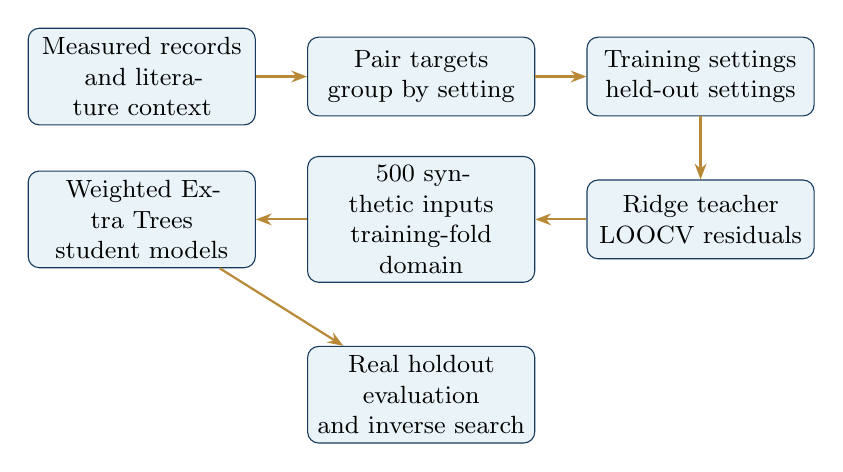
\begin{tikzpicture}[
  node distance=0.8cm and 0.65cm,
  box/.style={draw=IITNavy,rounded corners,fill=SoftBlue,align=center,text width=2.65cm,minimum height=1.0cm,font=\small},
  arrow/.style={-{Stealth[length=2mm]},thick,draw=IITGold}
]
\node[box] (data) {Measured records\\and literature context};
\node[box,right=of data] (group) {Pair targets\\group by setting};
\node[box,right=of group] (split) {Training settings\\held-out settings};
\node[box,below=of split] (teacher) {Ridge teacher\\LOOCV residuals};
\node[box,left=of teacher] (augment) {500 synthetic inputs\\training-fold domain};
\node[box,left=of augment] (student) {Weighted Extra Trees\\student models};
\node[box,below=of augment] (eval) {Real holdout evaluation\\and inverse search};
\draw[arrow] (data)--(group);
\draw[arrow] (group)--(split);
\draw[arrow] (split)--(teacher);
\draw[arrow] (teacher)--(augment);
\draw[arrow] (augment)--(student);
\draw[arrow] (student)--(eval);
\end{tikzpicture}
\caption{Grouped, leakage-aware workflow used in the current joint-property study.}
\label{fig:updated-methodology}
\end{figure}

\section{Evaluation strategy}
Evaluation is reported at three levels. First, training-only leave-one-condition-out predictions provide a diagnostic of how the Ridge teacher extrapolates to a held-out measured condition among the training settings. Second, the validation-fold student models are evaluated on the two preselected real held-out settings. Third, the inverse workflow uses the validation-only models to test whether a target property vector can lead back to a known setting. These checks answer different questions and are reported separately.

The metrics include mean squared error (MSE), root mean squared error (RMSE), mean absolute error (MAE), coefficient of determination ($R^2$), and mean absolute percentage error (MAPE). MSE is reported in squared property units; RMSE and MAE retain the property units. With only two independent held-out settings, holdout $R^2$ is included as a descriptive statistic only and should not be interpreted as a stable estimate of generalization performance.

\chapter{Experimental Setup and Characterization}

\section{LPBF fabrication context}
The Haynes 282 samples were fabricated on an EOS M-series LPBF system at the Precision Engineering Hub, IIT (BHU), Varanasi. The process parameters paired to the current mechanical-property measurements are laser power, scan speed, hatch distance, and layer thickness. All settings in the present 20-record mechanical-property table use a layer thickness of \SI{0.04}{mm}. The wider parameter ranges reported in Part I describe the broader modeling context and should not be interpreted as the coverage of the current small experimental campaign.

\begin{figure}[H]
\centering
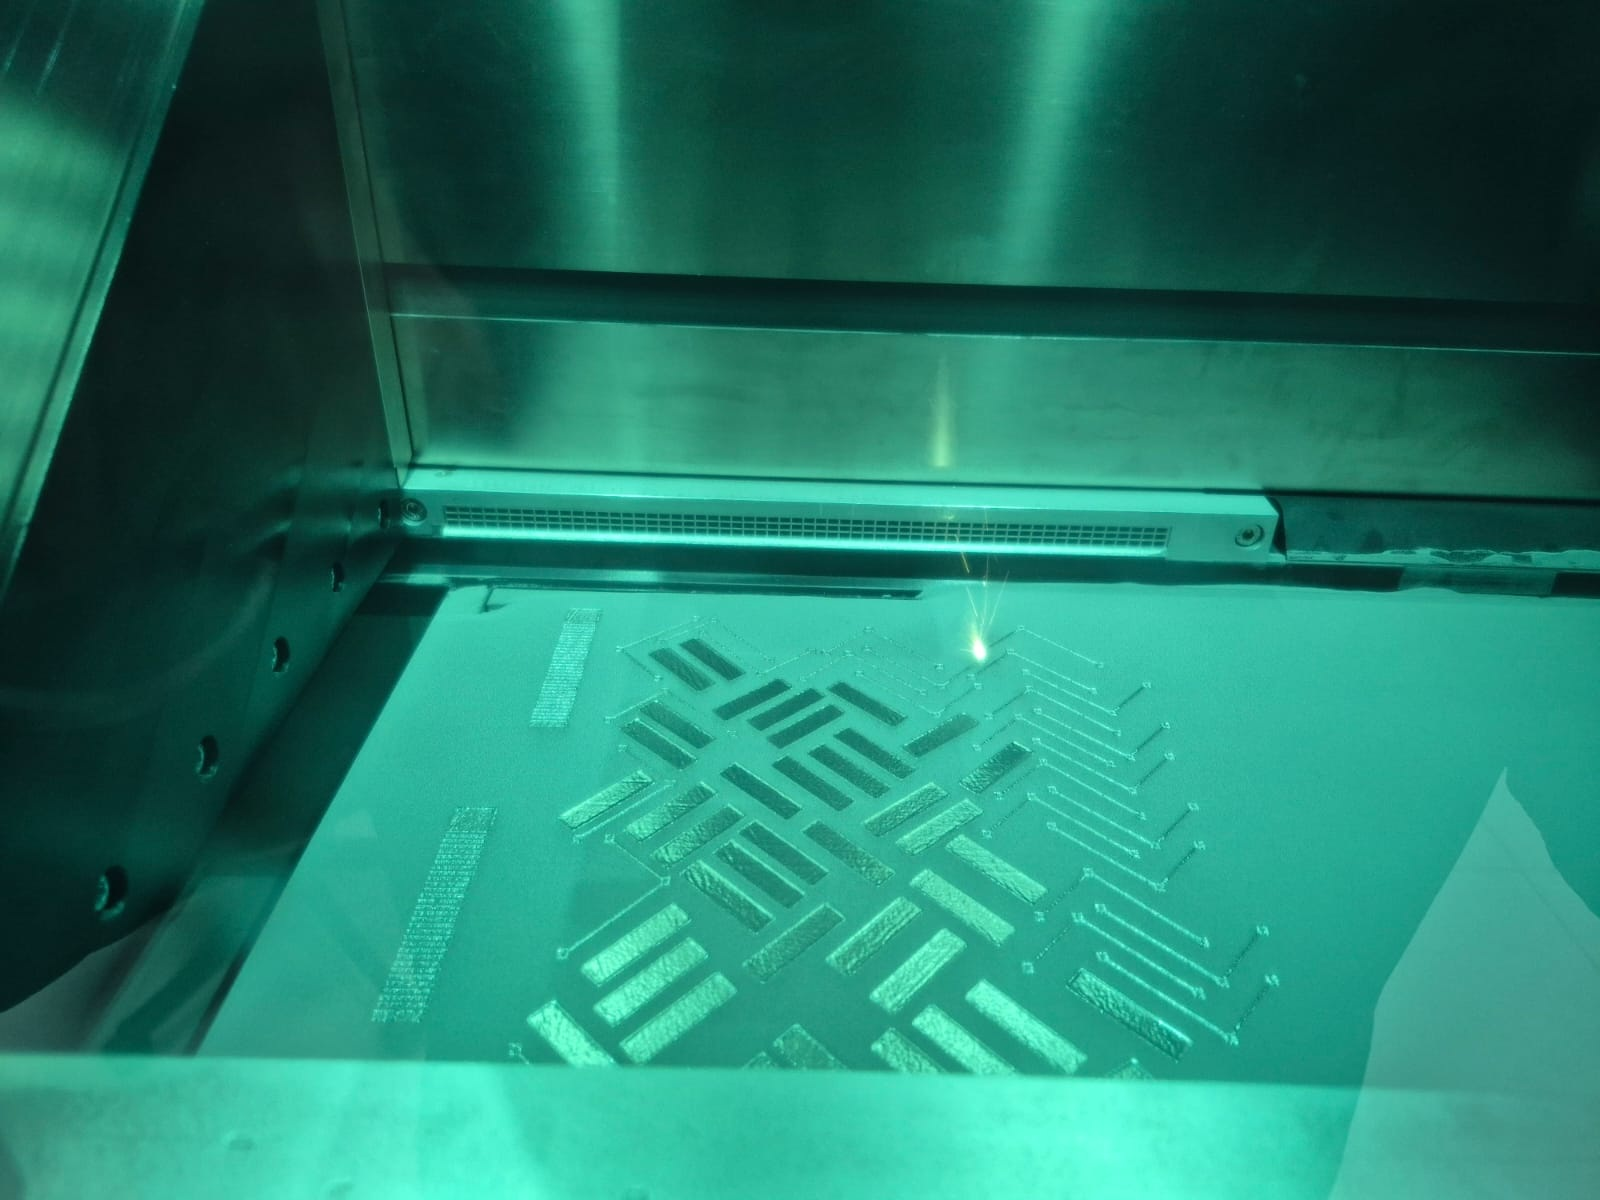
\includegraphics[width=0.72\textwidth]{printing_live.jpg}
\caption{LPBF build in progress. Replace or supplement this image with a labelled build-plate view if a closer sample-specific image is available.}
\label{fig:printing-live}
\end{figure}

\section{Tensile testing for UTS}
Tensile specimens were tested using the Tinius Olsen H25KL frame. The load train and mounted specimen are shown in Figure~\ref{fig:uts-frame}. The UTS values in the experimental table are treated as measured outputs paired with their recorded process settings. The available records do not specify the tensile standard, specimen geometry, gauge dimensions, test temperature, strain rate, extensometer configuration, or number of tensile replicates for each condition. These protocol details must be confirmed from laboratory records before final submission; they are not inferred from the equipment photograph.

\begin{figure}[H]
\centering
\begin{subfigure}[t]{0.45\textwidth}
\centering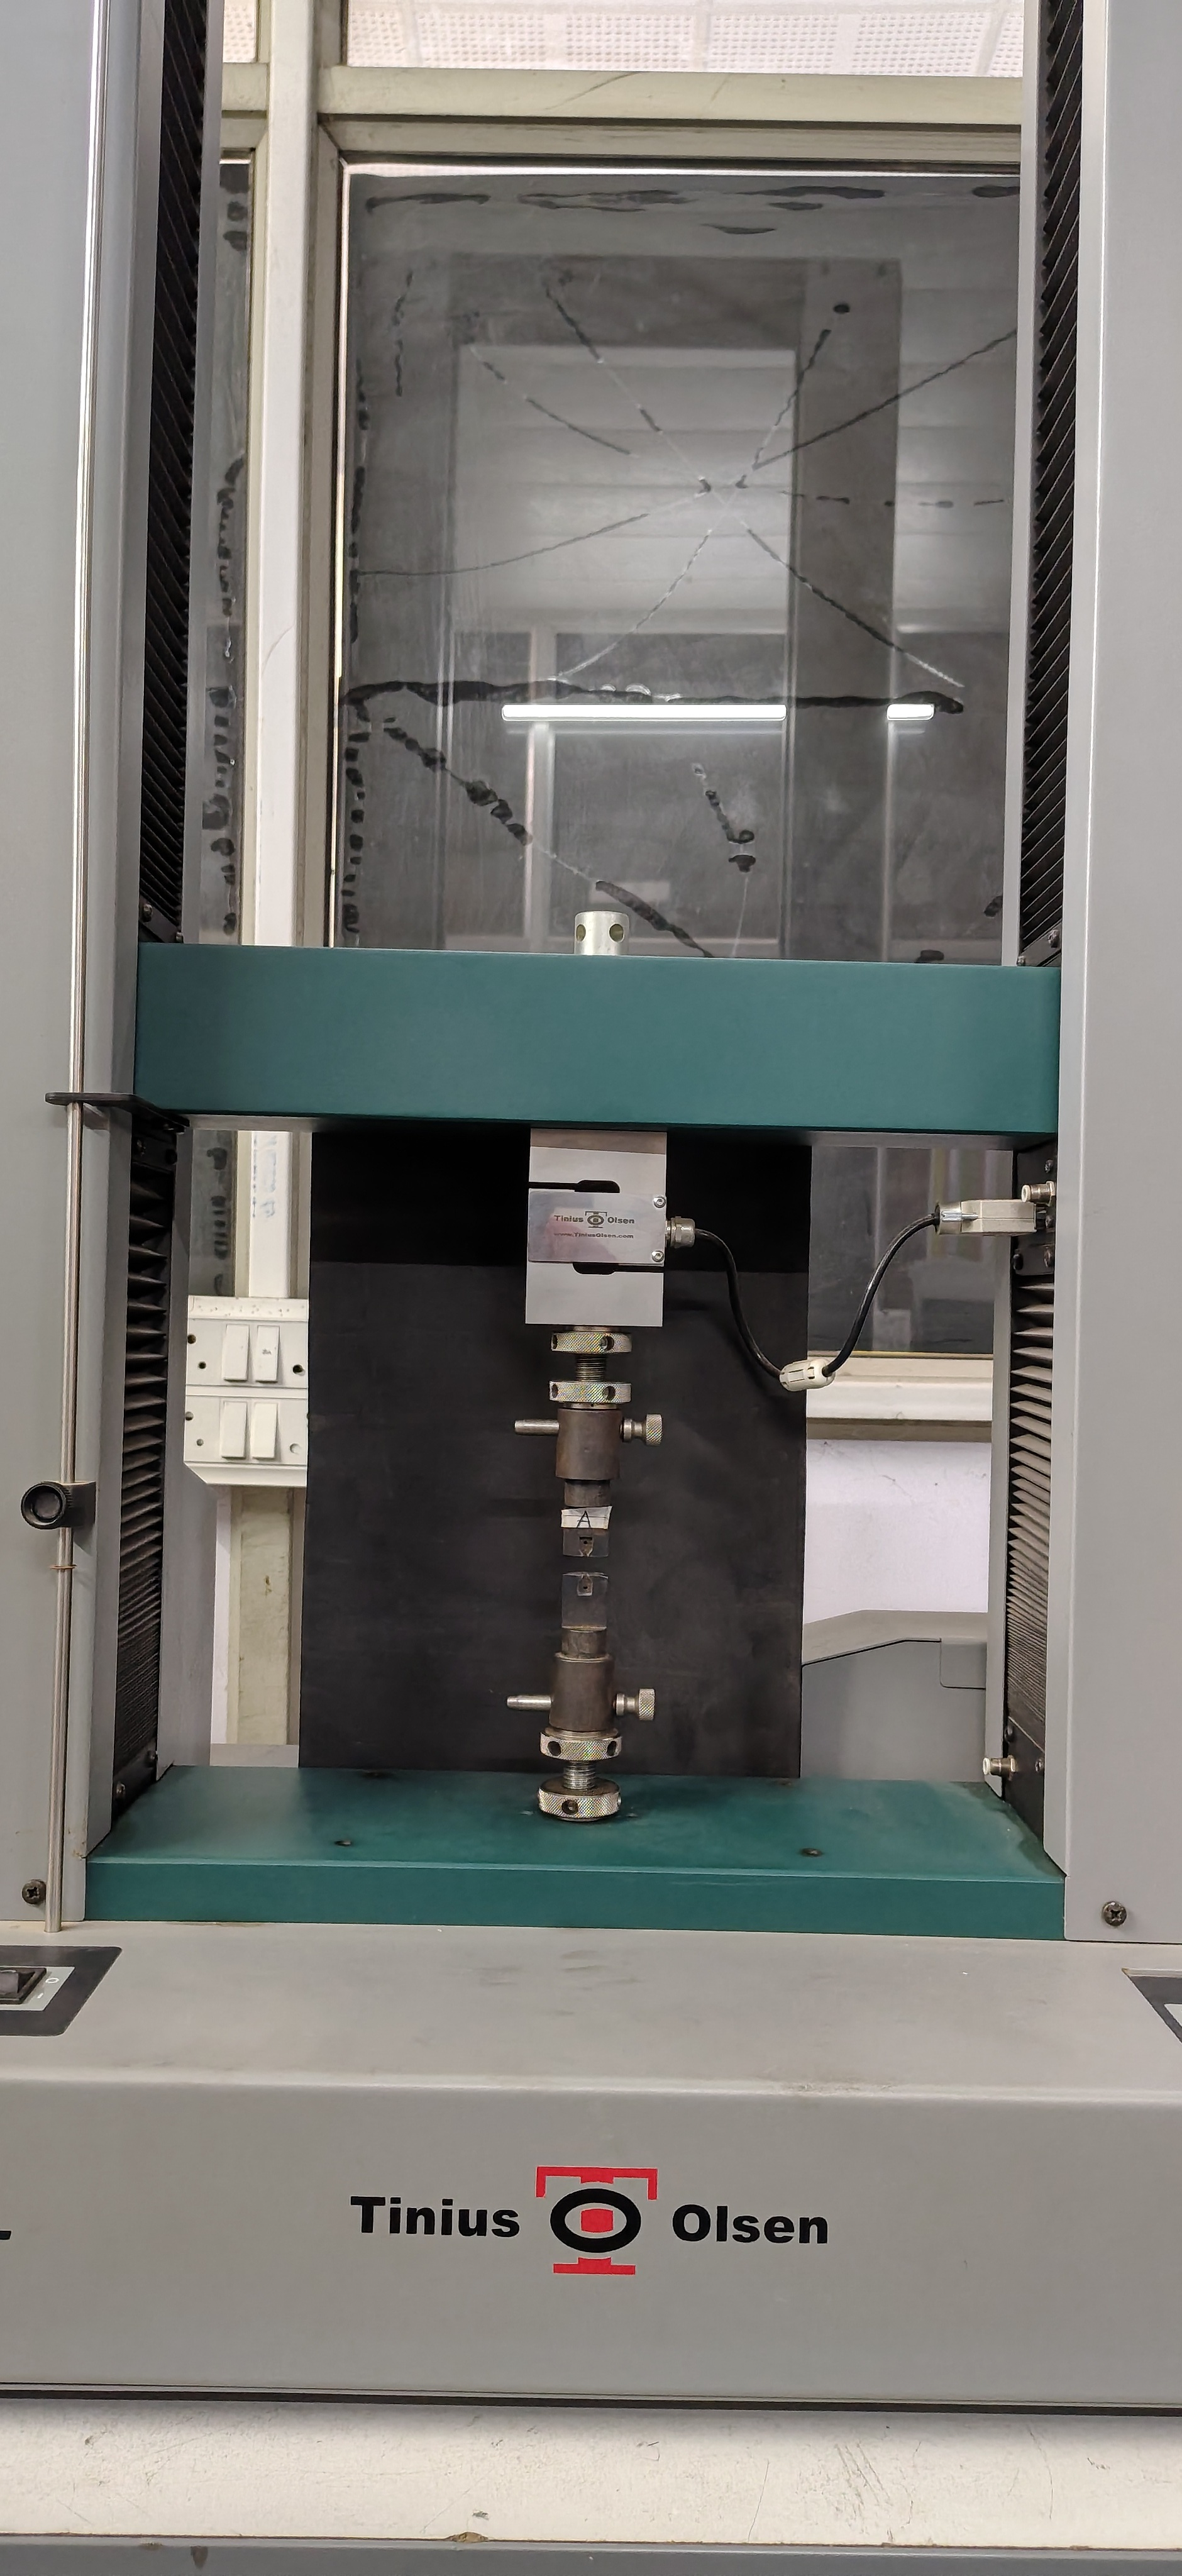
\includegraphics[height=7.1cm,keepaspectratio]{tinius_olsen_setup.jpg}
\caption{Mounted tensile specimen and load train.}
\end{subfigure}\hfill
\begin{subfigure}[t]{0.45\textwidth}
\centering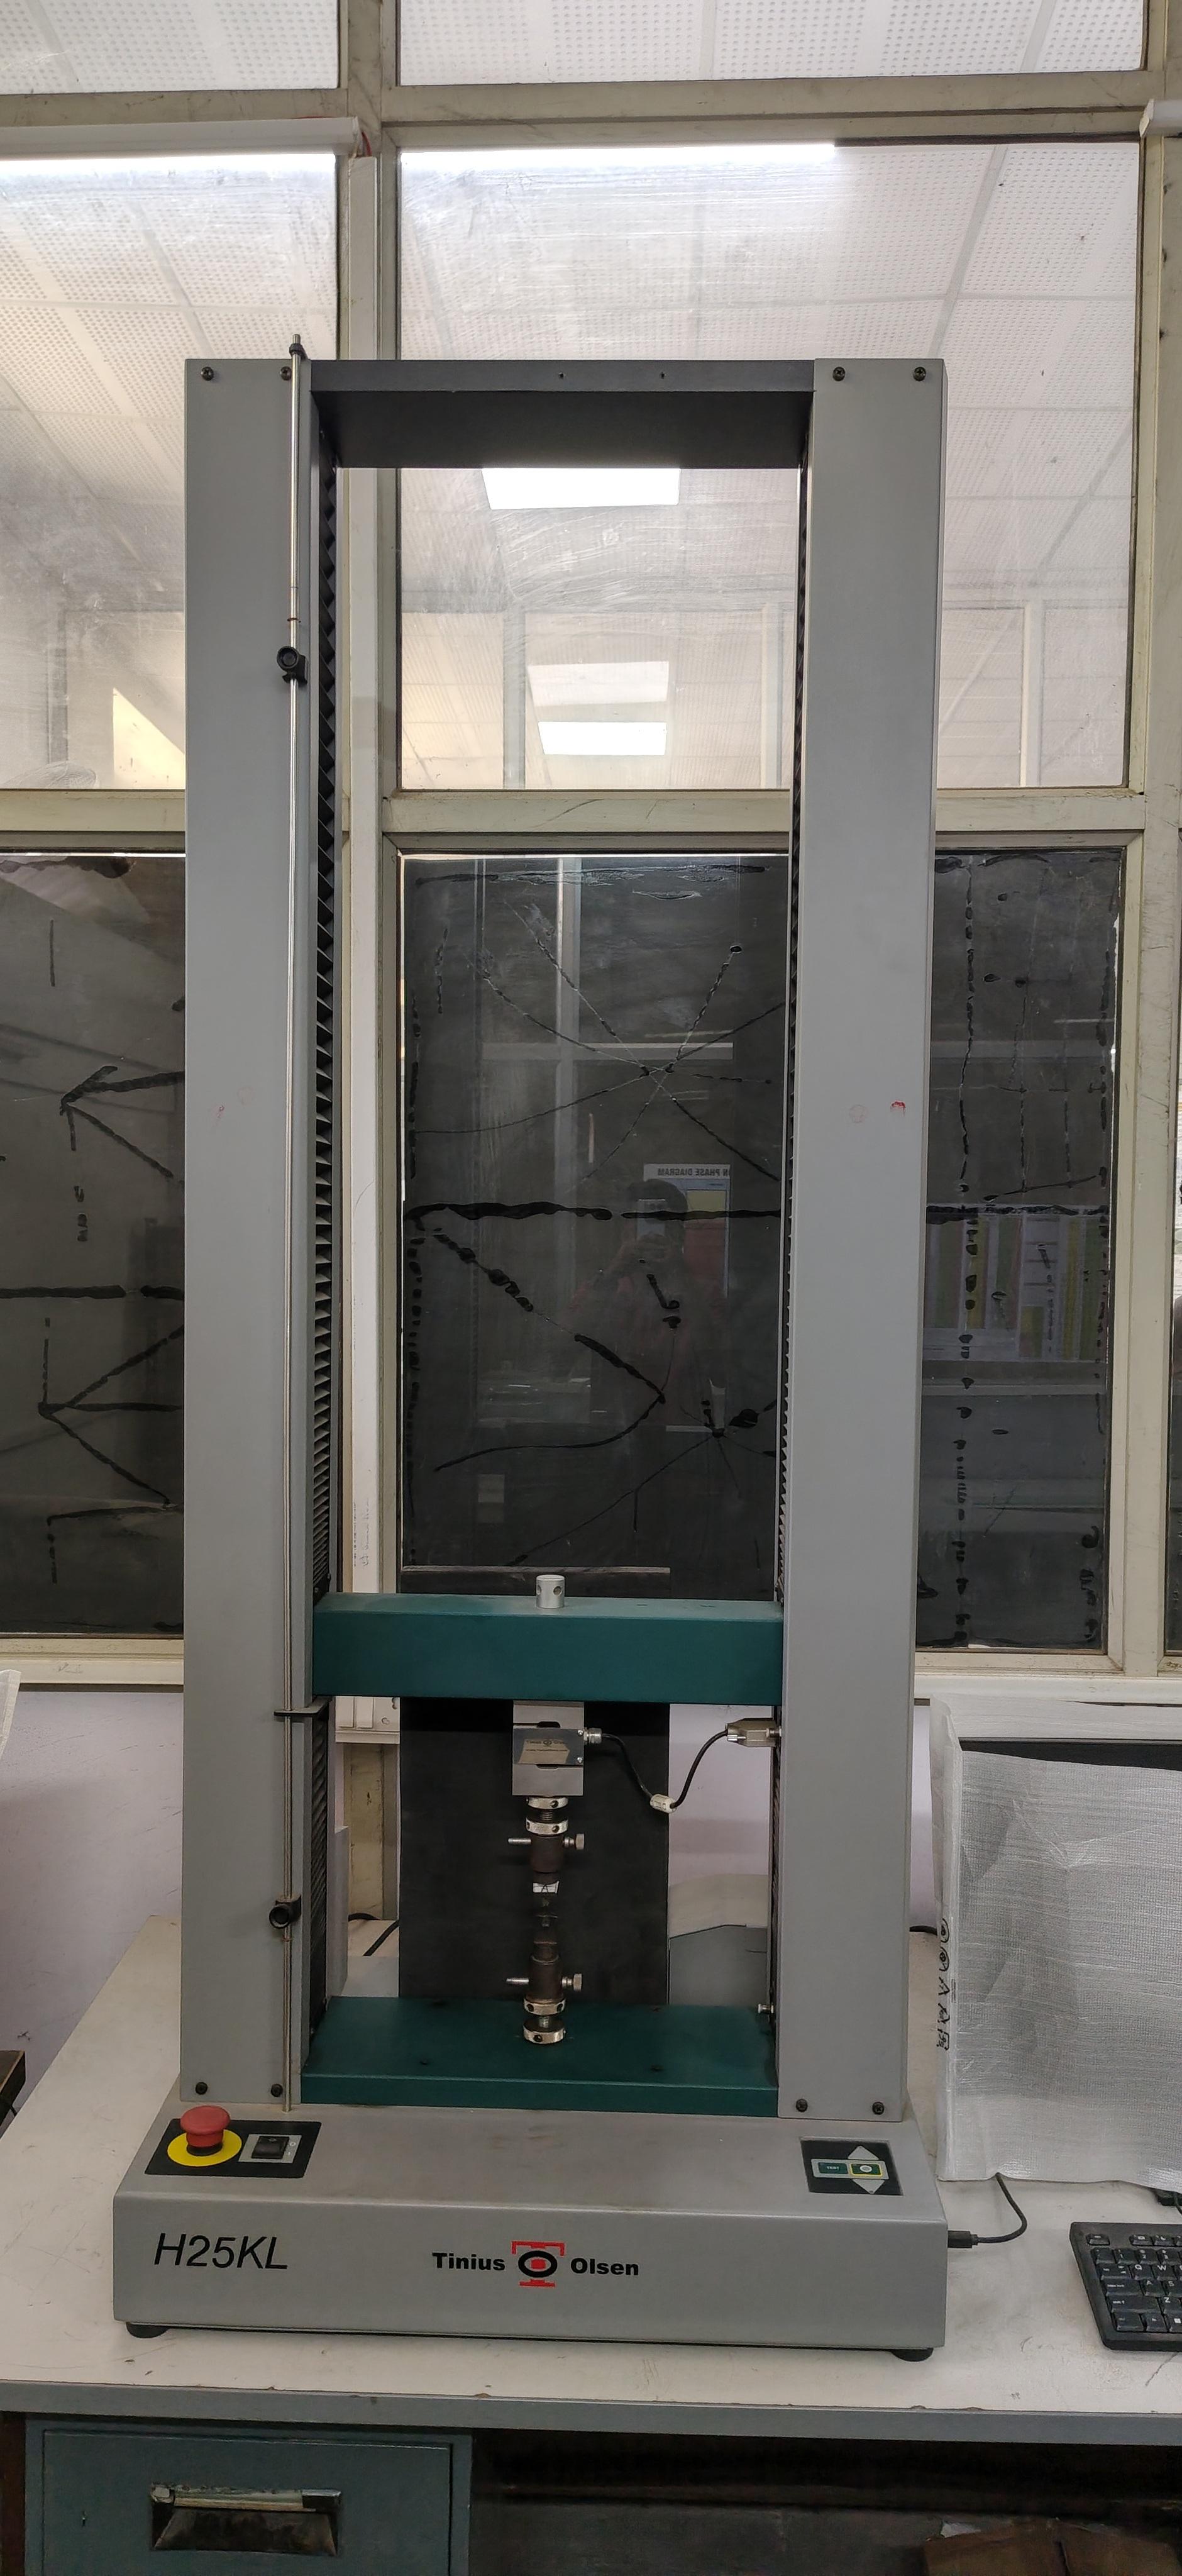
\includegraphics[height=7.1cm,keepaspectratio]{tinius_olsen_full.jpg}
\caption{Tinius Olsen H25KL frame.}
\end{subfigure}
\caption{Experimental tensile-test setup used for UTS characterization.}
\label{fig:uts-frame}
\end{figure}

\noindent\textbf{Protocol information to complete:} tensile test standard; specimen dimensions and build orientation; test temperature; loading or strain rate; extensometer details; number of specimens per process setting; and the rule used to select the reported UTS where repeats exist.

\section{Hardness testing}
Hardness was measured using a Mitutoyo HM-200 tester with an optical microscope for locating and reading indentations (Figure~\ref{fig:hardness-setup}). Each sample record contains six perpendicular readings and three parallel readings. The two orientation means are averaged with equal weight to create the composite hardness target in HV. This equal-orientation rule prevents the group with more indent readings from automatically receiving greater weight.

\begin{figure}[H]
\centering
\begin{subfigure}[t]{0.45\textwidth}
\centering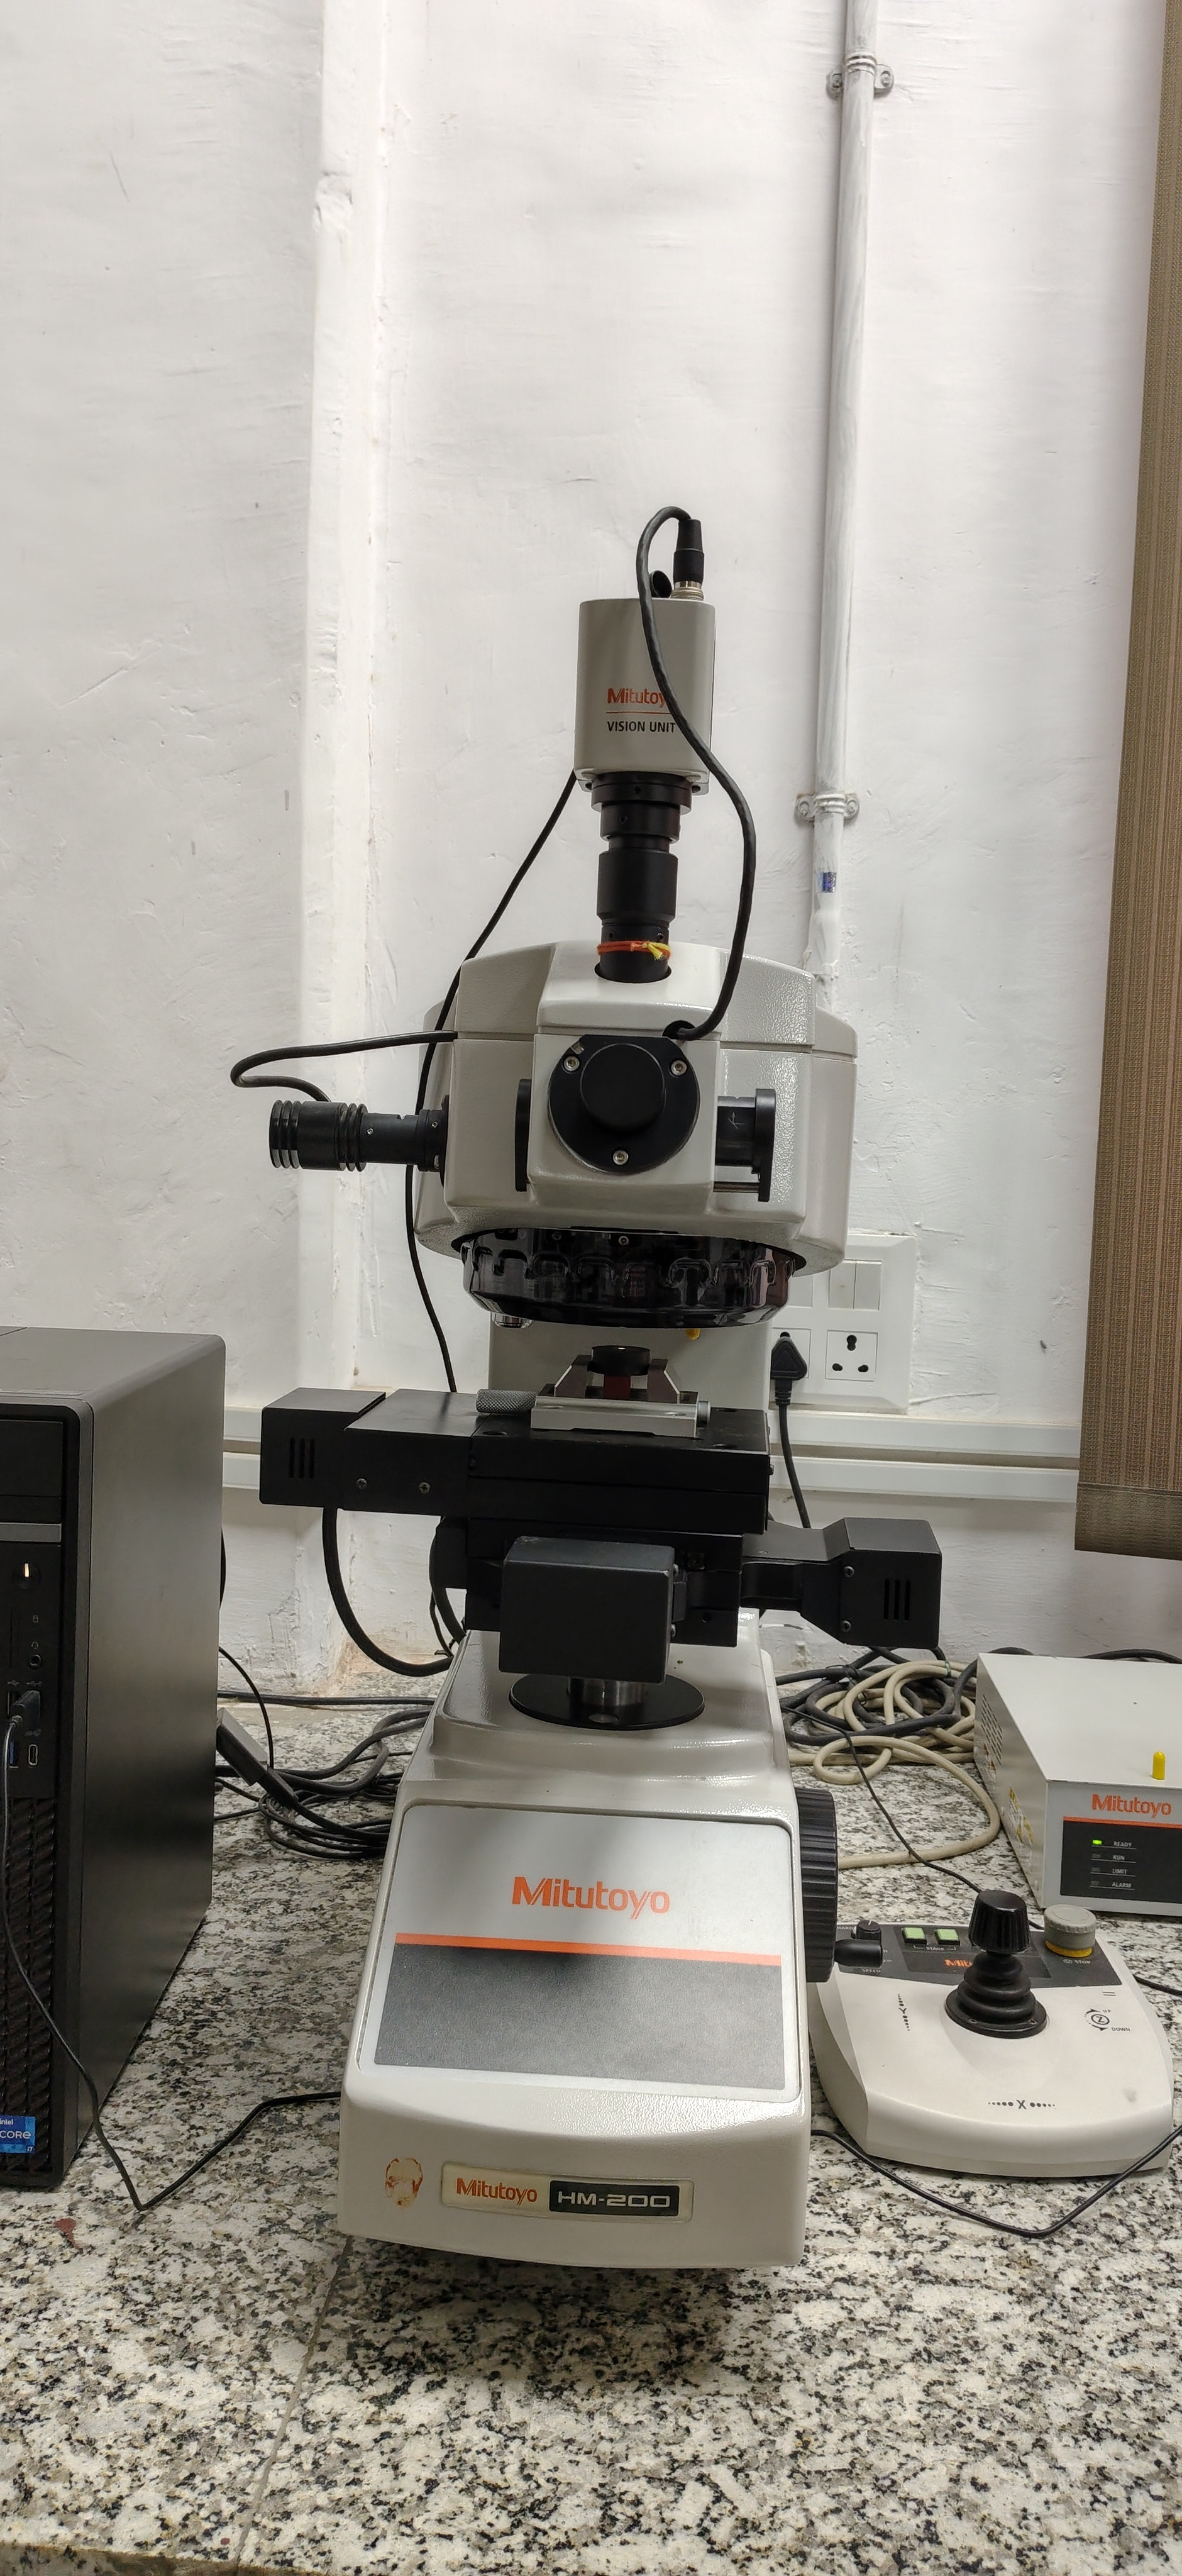
\includegraphics[height=7.2cm,keepaspectratio]{mitutoyo_hm200.jpg}
\caption{Mitutoyo HM-200 hardness tester.}
\end{subfigure}\hfill
\begin{subfigure}[t]{0.45\textwidth}
\centering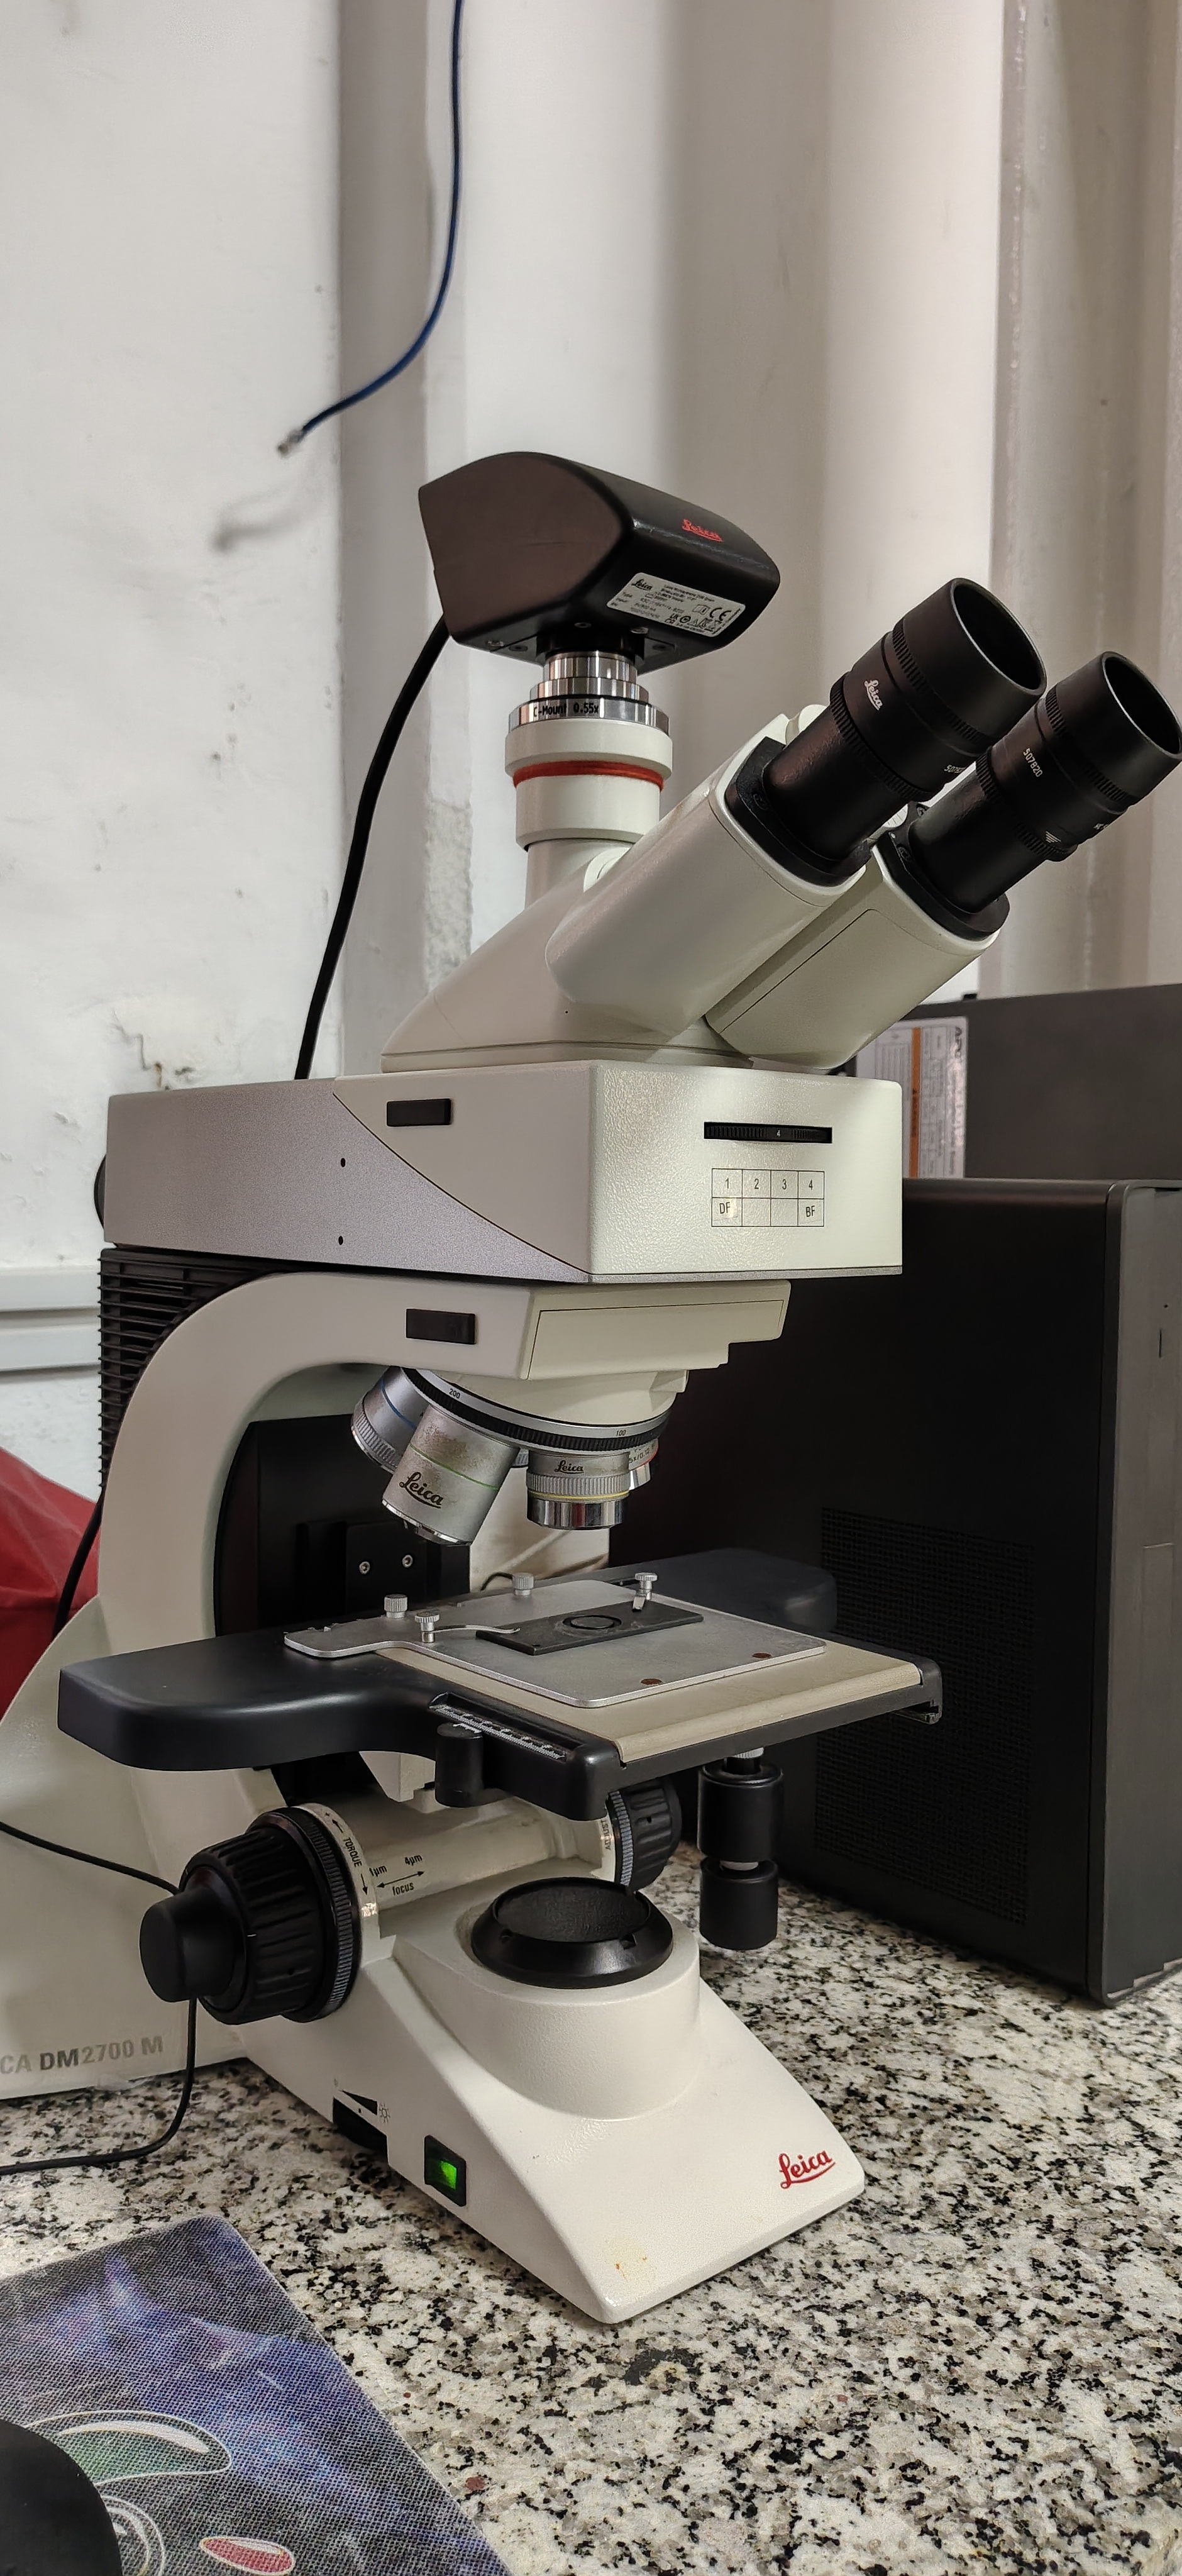
\includegraphics[height=7.2cm,keepaspectratio]{hardness_microscope.jpg}
\caption{Optical microscope used to inspect indentation marks.}
\end{subfigure}
\caption{Hardness measurement equipment.}
\label{fig:hardness-setup}
\end{figure}

The available workbook identifies the readings as HV, but the test force, dwell time, indenter specification, surface preparation, and applicable test standard were not present in the supplied table. These values should be verified from the instrument logs or laboratory notebook. They are intentionally left as completion items in this draft.

\section{Relative-density measurements}
Relative density was measured using the Archimedes method described in the first report. The current experimental table stores relative density in percent, whereas the legacy model artifacts may use fractional density. This report uses percentage units consistently for the joint model outputs. The density value associated with sample 11 must be reconciled before submission: the current working CSV contains \SI{99.95}{\percent}, while the Part I presentation table reports \SI{99.45}{\percent}. The calculations in this continuation use the current working CSV value and should be updated if the laboratory record confirms a different measurement.

\section{Hardness aggregation example}
Table~\ref{tab:hardness-repeat-summary} summarizes the six-repeat validation condition. The standard deviation describes sample-to-sample variability in the composite hardness values; it is not the standard error of the fitted model.
\begin{table}[H]
\centering
\caption{Hardness repeatability at the six-replicate validation setting.}
\label{tab:hardness-repeat-summary}
\begin{tabular}{lrrrr}
\toprule
Power (W) & Speed (mm/s) & Hatch (mm) & Mean hardness (HV) & Sample SD (HV)\\
\midrule
270 & 1500 & 0.080 & 324.90 & 3.55\\
\bottomrule
\end{tabular}
\end{table}

\chapter{Data Preparation and Model Development}

\section{Measured property table}
The hardness workbook contributes 20 sample-level hardness composites. The UTS/density table contributes corresponding values for the same sample identifiers. The rows represent 15 unique process settings because six records share one setting and several settings have repeated conditions elsewhere. Before fitting, targets are aligned by sample identifier and then grouped by all four process inputs. A consistency assertion confirms that each process condition belongs entirely to one split.

The training and validation split is fixed by setting rather than by individual row. The repeated group at $(270,1500,0.08,0.04)$ and sample 11 at $(280,1550,0.085,0.04)$ form the two held-out conditions. This leaves 13 unique settings for training. In the forward holdout report, the six-repeat group is represented by its measured mean and standard deviation; it remains one independent process setting, not six independent validation settings.

\begin{table}[H]
\centering
\caption{Targets and units used by the joint forward and inverse models.}
\label{tab:targets}
\begin{tabular}{lll}
\toprule
Target column & Reported unit & Aggregation\\
\midrule
Hardness\_HV & HV & Mean of orientation means, then process-condition mean\\
UTS\_MPa & MPa & Process-condition mean where repeats are present\\
RelativeDensity\_pct & \% & Process-condition mean where repeats are present\\
\bottomrule
\end{tabular}
\end{table}

\section{Synthetic augmentation}
The term ``500 points'' has two meanings in the project history and they must not be conflated. Part I describes a broad 500-row dataset used for preliminary model comparisons. The current joint pipeline creates a separate 500-row synthetic augmentation set for a given fit. In the validation fold, that synthetic set is generated only from the training conditions and their training-fold teachers. It does not contain new independent physical measurements. After validation, the final models are refit on all measured conditions and a fresh synthetic set is generated for candidate search.

The teacher model is a standardized Ridge regression with regularization parameter $\alpha=10$. Out-of-fold teacher residuals are centred and resampled with replacement to perturb the synthetic predictions. The student is an Extra Trees regressor with 300 trees, maximum depth 6, minimum leaf size 2, maximum feature fraction 0.8, and fixed random seed 42. Sample weights give the measured condition means an aggregate weight comparable to the synthetic augmentation set. The student architecture is fixed in the current implementation; its reported real-setting validation is therefore more informative than a random train/test split over generated rows.

\section{Training-only cross-validation}
Leave-one-condition-out (LOOCV) is applied to the 13 training settings for each property. The teacher is refit on 12 conditions in each fold, and the left-out measured value is predicted. This procedure yields one out-of-fold estimate per training setting. It does not evaluate the final student on an independent external dataset and should be labelled ``training-only LOOCV diagnostic'' in figures and tables.

\section{Validation-fold exclusion}
For each held-out process setting, none of its records or target values participate in teacher fitting, residual estimation, synthetic augmentation, student fitting, target scaling, or validation-fold search bounds. The measured properties at the held-out input are compared with predictions from the validation-fold student. The final models used for Pareto search are subsequently trained on all 15 unique settings; performance on those final models is not reported as held-out accuracy.

\chapter{Results}

\section{Training-only LOOCV diagnostics}
Table~\ref{tab:loocv} reports out-of-fold errors for the Ridge teachers on the 13 training settings. The negative $R^2$ values mean that the LOOCV predictions do not outperform the baseline that predicts the mean target value for every held-out setting. This is an important limitation, particularly for UTS and hardness, and argues for adding more unique process conditions before making strong generalization claims.

\begin{table}[H]
\centering
\caption{Training-only LOOCV diagnostics for Ridge teachers.}
\label{tab:loocv}
\begin{tabular}{lrrrrrr}
\toprule
Property & $n$ & MSE & RMSE & MAE & $R^2$ & MAPE (\%)\\
\midrule
UTS (MPa) & 13 & 1500.85 & 38.74 & 27.02 & -0.305 & 3.11\\
Density (percentage points) & 13 & 0.2260 & 0.4754 & 0.3479 & -0.062 & 0.351\\
Hardness (HV) & 13 & 54.60 & 7.39 & 6.24 & -0.347 & 1.92\\
\bottomrule
\end{tabular}
\end{table}

RMSE and MAE are expressed in the original property units. Density errors are percentage points: for example, a change from \SI{99.5}{\percent} to \SI{99.0}{\percent} is an error of 0.5 percentage points. MAPE expresses absolute errors relative to the measured values. Because these properties have very different scales, raw MSE values should not be compared across columns.

\section{Forward prediction at the two held-out settings}
The forward validation asks whether the models can predict the measured properties at known process settings. Table~\ref{tab:forward-holdout} gives measured means, predictions, and signed percentage error. The six-repeat group has a measured mean UTS of \SI{890}{MPa}, density of \SI{99.617}{\percent}, and composite hardness of \SI{324.90}{HV}. Sample 11 has measured values of \SI{923}{MPa}, \SI{99.95}{\percent} in the current CSV, and \SI{323.38}{HV}.

\begin{table}[H]
\centering
\caption{Forward-model validation on the grouped held-out settings.}
\label{tab:forward-holdout}
\begin{tabular}{llrrrr}
\toprule
Setting & Property & Measured & Predicted & Error & Error (\%)\\
\midrule
Six repeats & Hardness (HV) & 324.90 & 328.31 & +3.42 & +1.051\\
Six repeats & UTS (MPa) & 890.00 & 902.48 & +12.48 & +1.402\\
Six repeats & Density (\%) & 99.617 & 99.450 & -0.167 & -0.168\\
Sample 11 & Hardness (HV) & 323.38 & 322.47 & -0.90 & -0.280\\
Sample 11 & UTS (MPa) & 923.00 & 875.13 & -47.87 & -5.186\\
Sample 11 & Density (\%) & 99.950 & 99.591 & -0.359 & -0.359\\
\bottomrule
\end{tabular}
\end{table}

The strongest holdout miss is UTS at sample 11, with a signed error of approximately $-5.19\%$. The density discrepancy is small in absolute percentage points, but the conflict between the current density CSV and the Part I table must be reconciled before presenting this value as final. The forward results are encouraging for the repeated condition but are not sufficient to characterize broad process-space generalization because only two independent settings are held out.

\begin{figure}[H]
\centering
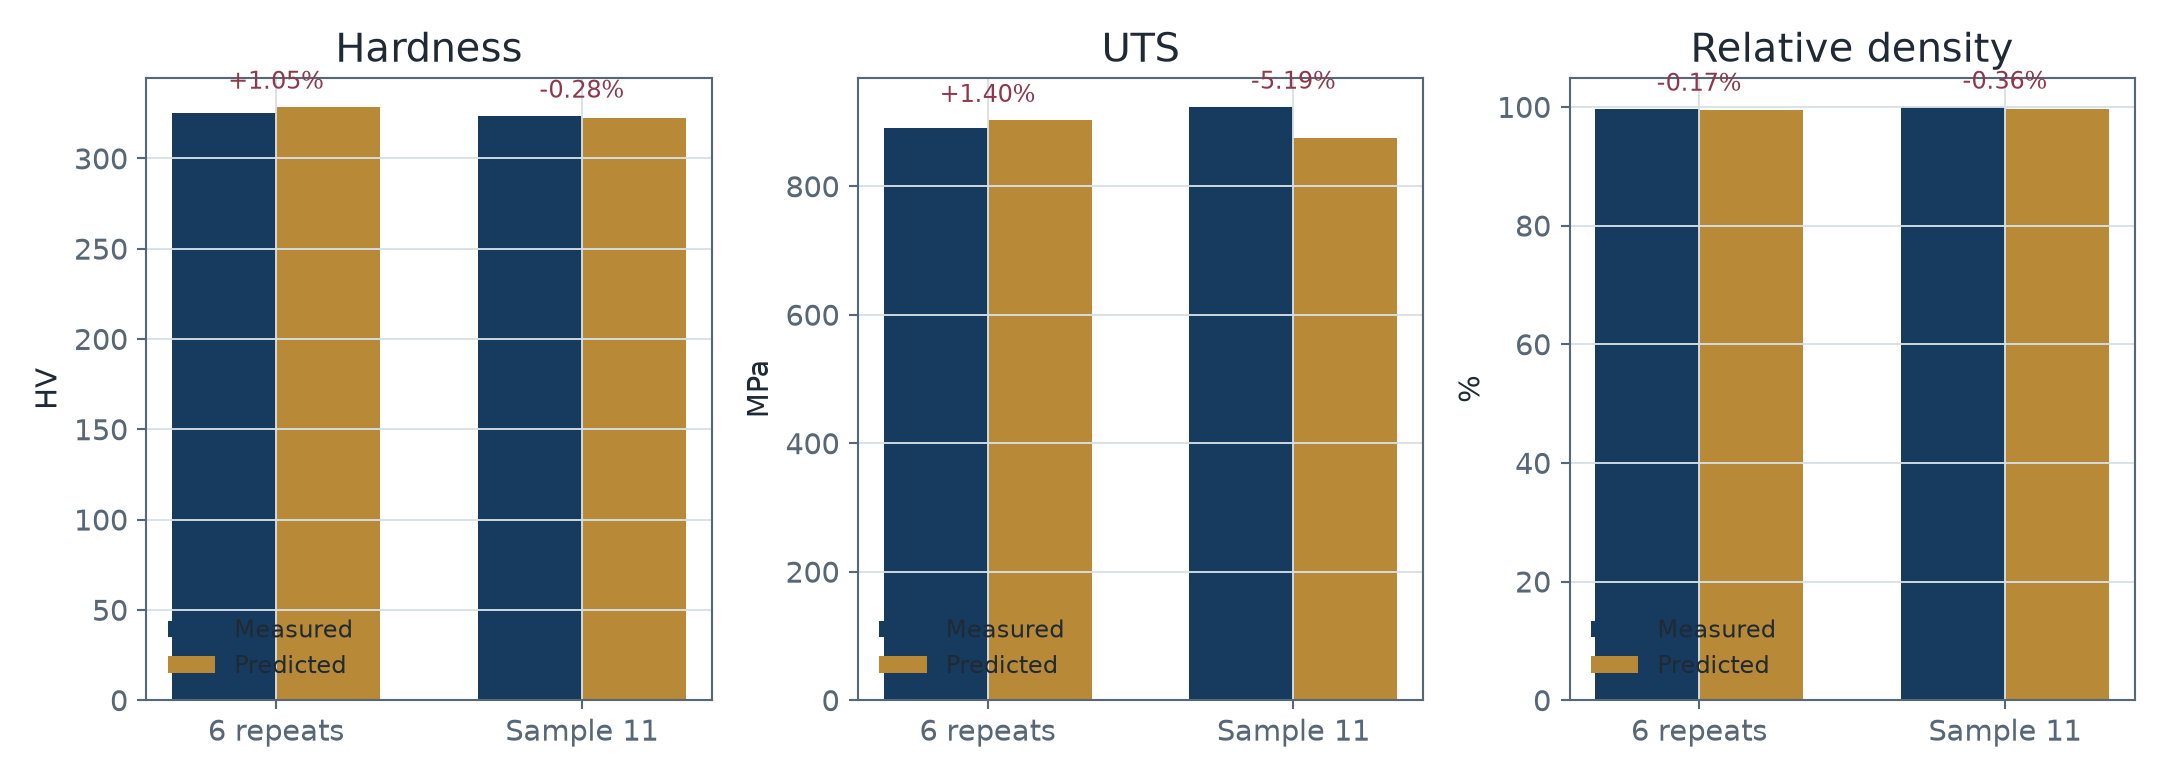
\includegraphics[width=0.95\textwidth]{holdout_actual_predicted.png}
\caption{Measured and predicted values at the two held-out settings. Error annotations show signed percentage error relative to measurement.}
\label{fig:holdout-bars}
\end{figure}

\section{Inverse recovery evaluation}
The inverse evaluation asks a different question: given the measured property vector at a held-out condition, can the validation-fold inverse search recover that process setting? The optimizer is allowed to find a different setting if the forward surrogate predicts similar properties. Therefore, a close property match does not imply recovery of the original parameters.

\begin{table}[H]
\centering
\caption{Inverse recovery results using models trained without either held-out setting.}
\label{tab:inverse-recovery}
\small
\begin{tabular}{lrrrrrr}
\toprule
Target setting & Actual $(P,v,h)$ & Recovered $(P,v,h)$ & Hardness error & UTS error & Density error\\
\midrule
Six repeats & (270, 1500, 0.080) & (280.2, 1534.2, 0.0788) & -0.022\% & -0.222\% & +0.0001\%\\
Sample 11 & (280, 1550, 0.085) & (270.2, 1420.8, 0.0900) & -0.303\% & -2.151\% & -0.270\%\\
\bottomrule
\end{tabular}
\end{table}

For the six-repeat setting, the inverse search found a different parameter combination with nearly identical predicted properties. This is evidence of non-uniqueness: several process settings can map to a similar property vector under the surrogate. For sample 11, inverse recovery is weaker, particularly for UTS. Neither inverse result substitutes for a physical build at the recommended setting.

\begin{figure}[H]
\centering
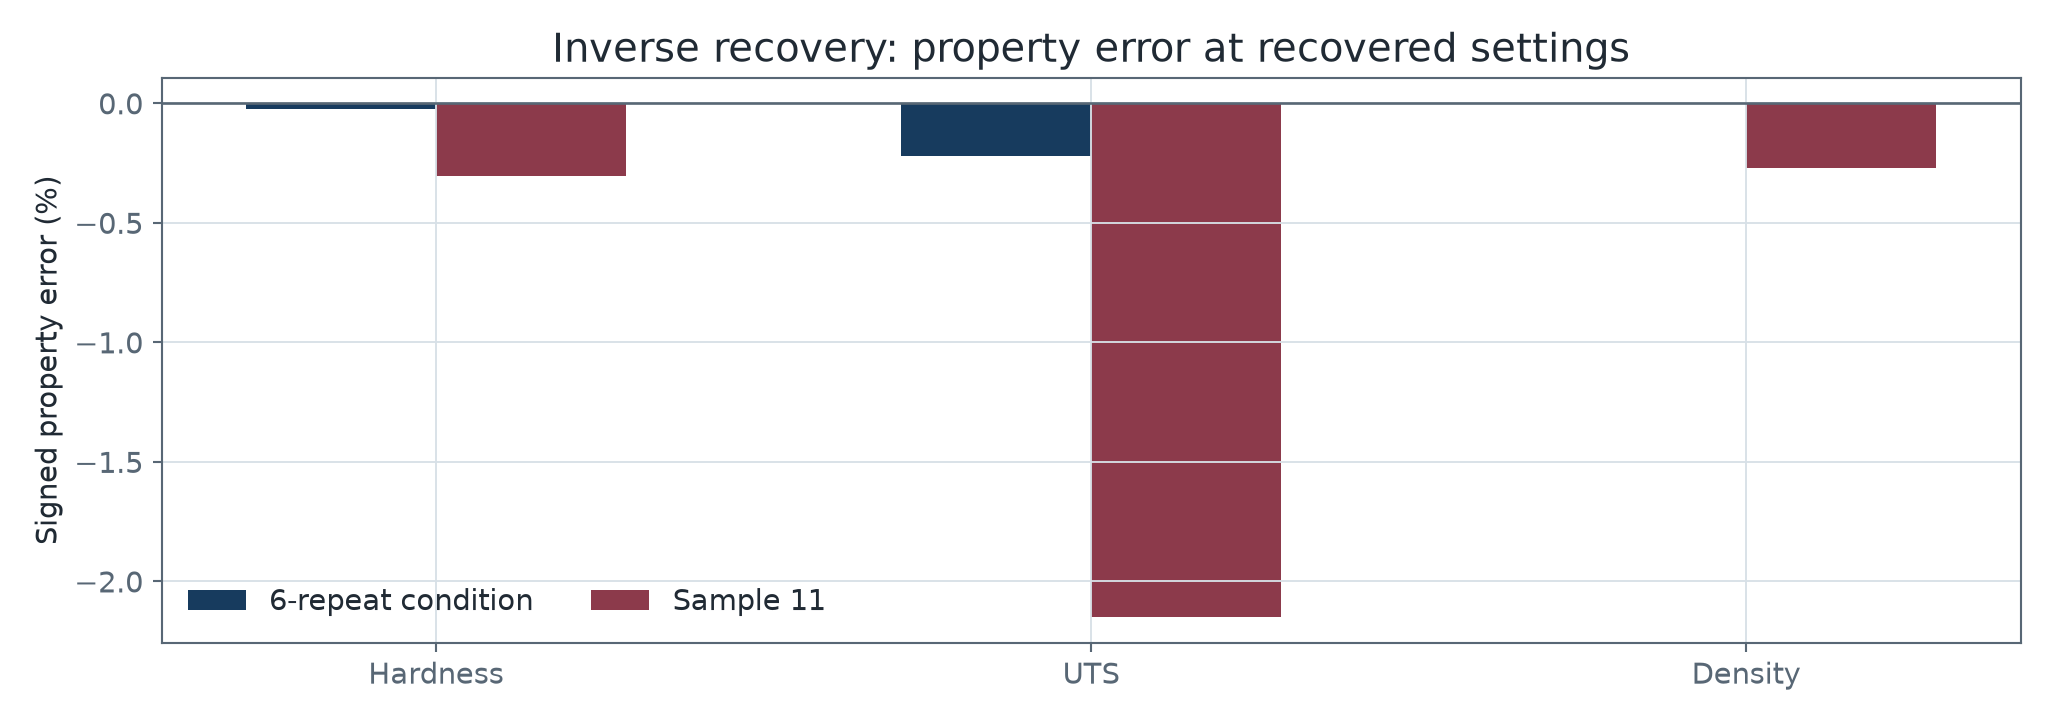
\includegraphics[width=0.88\textwidth]{inverse_property_errors.png}
\caption{Signed property errors in the inverse recovery exercise.}
\label{fig:inverse-error}
\end{figure}

\section{Pareto candidate set}
A three-objective NSGA-II search was conducted over the measured parameter bounds and the observed volumetric-energy-density window. The final models used for this search were refit on all 15 unique measured settings and their final augmentation set. The six selected candidates are non-dominated trade-offs and were further selected for parameter-space diversity. They are screening candidates, not experimentally validated recipes.

\begin{table}[H]
\centering
\caption{Six diverse Pareto candidates for experimental follow-up.}
\label{tab:pareto}
\small
\begin{tabular}{rrrrrrr}
\toprule
Candidate & Power (W) & Speed (mm/s) & Hatch (mm) & VED (J/mm$^3$) & Hardness (HV) & UTS (MPa) / Density (\%)\\
\midrule
1 & 268.2 & 1402 & 0.0799 & 59.89 & 331.47 & 905.2 / 99.771\\
2 & 286.0 & 1409 & 0.0796 & 63.74 & 328.18 & 892.9 / 99.805\\
3 & 251.8 & 1582 & 0.0701 & 56.78 & 327.15 & 931.2 / 99.144\\
4 & 273.8 & 1584 & 0.0710 & 60.83 & 327.83 & 905.7 / 99.328\\
5 & 262.4 & 1526 & 0.0784 & 54.83 & 326.94 & 907.9 / 99.370\\
6 & 270.9 & 1554 & 0.0882 & 49.44 & 322.17 & 910.3 / 99.534\\
\bottomrule
\end{tabular}
\end{table}

Candidate 1 leads the shortlist in hardness, candidate 3 in UTS, and candidate 2 in density. No one candidate maximizes all three objectives simultaneously. Before fabrication, parameter precision must be rounded to EOS machine increments and feasibility rechecked using the rounded values.

\chapter{Joint Inverse Optimization Interface}

\section{Interface design}
The Streamlit interface provides four views: forward prediction, inverse target search, saved Pareto candidates, and validation diagnostics. The forward view accepts power, speed, and hatch distance, while layer thickness is fixed to the trained model setting. It reports predicted hardness, UTS, relative density, and calculated volumetric energy density. A warning is shown when a setting is within individual parameter bounds but outside the observed VED window.

The inverse view accepts target hardness, UTS, and density, then minimizes equal-weight normalized squared target error while respecting the measured process domain and energy-density window. The output includes the recommended setting, property predictions, signed property errors, and a downloadable result table. The Pareto view displays the six non-dominated candidates. The validation view displays real held-out predictions and training-only LOOCV metrics. All predicted outputs are explicitly identified as surrogate estimates requiring experimental confirmation.

\section{User-interface testing}
The interface was checked in Streamlit's application test harness and in a local browser. The four expected tabs render: Forward prediction, Inverse targets, Pareto candidates, and Validation. The app uses the new joint artifacts trained in the project environment. The QR code and interface URL are intentionally left for the authors to add after selecting the deployment address.

\begin{figure}[H]
\centering
\fbox{\begin{minipage}[c][6.0cm][c]{0.88\textwidth}\centering\Large\color{Muted}Add final application screenshot here\\[0.8em]\normalsize Include the live URL or a QR code after deployment.\end{minipage}}
\caption{Reserved space for the final deployed UI screenshot and access QR code.}
\label{fig:ui-placeholder}
\end{figure}

\section{Suggested acceptance checks}
Before release, the authors should test a known measured condition in forward mode, verify target-property error columns in inverse mode, confirm that out-of-window VED is clearly flagged, download CSV results, and compare the saved Pareto table with the current model version. The UI should not describe candidates as certified process recipes. A build-and-test loop remains necessary.

\chapter{Discussion and Limitations}

\section{What the current results support}
The current work supports a reproducible integration of measured hardness, UTS, and density with a grouped training/validation workflow. It also demonstrates how a small measured set can be expanded into a model-guided candidate search while preserving the original real observations as weighted anchors. The six-repeat condition offers information about repeatability at one process setting, and sample 11 provides a second setting for a preliminary transfer check.

The inverse exercise illustrates that the property-to-process map can be many-to-one. The six-repeat target vector is matched by a different parameter combination, while sample 11 shows a larger UTS discrepancy. Therefore, inverse optimization should be interpreted as candidate generation under a particular surrogate and objective, rather than a unique inverse solution.

\section{Limitations}
The main limitations are the small number of unique measured settings, the limited number of held-out settings, and the dependence of synthetic labels on fitted teacher models. Synthetic augmentation improves coverage of the input domain but does not add independent physical evidence. Negative training-only LOOCV $R^2$ values show that teacher predictions do not beat a mean baseline on the current training settings. The reported two-setting holdout $R^2$ is highly unstable and should not be used as a headline metric.

The tensile test protocol details and hardness test force/dwell settings are not included in the supplied data. The current sample 11 density value differs between the working CSV and Part I report. These records must be reconciled and documented. The Pareto search operates within the measured bounds but predictions between sparse measured settings remain uncertain. Any future experiment should include process settings selected to reduce uncertainty, not only settings predicted to maximize the current point estimates.

\section{Recommended next experiments}
A useful next campaign would fabricate several distinct Pareto candidates and include at least one repeated condition to estimate measurement variability. Each new build should record actual machine setpoints, specimen orientation, test standard, tensile geometry and rate, hardness load and dwell, density measurement details, and any excluded or failed tests. The new measurements should be appended to the real-condition table before retraining. A larger set of unique process settings will improve both forward generalization and inverse identifiability.

\chapter{Conclusion and Future Work}
This continuation extends the Haynes 282 project from broad process-property modeling to a joint mechanical-property study using hardness, UTS, and relative density. A consistent table was assembled from the current experimental records, the hardness values were summarized across two orientations, and replicated process settings were grouped before model evaluation.

A Ridge-teacher/Extra-Trees-student pipeline was used with a training-fold synthetic augmentation set and real-condition anchors. Validation at two held-out settings shows mixed performance: the six-repeat condition is predicted within modest relative errors, while sample 11 has a notable UTS miss. Training-only LOOCV $R^2$ is negative for all three targets, so more unique real measurements are needed before the models can support strong generalization claims.

The inverse optimizer now supports target matching across three properties and multi-objective Pareto candidate generation. Its outputs provide a practical shortlist for future experiments, but the results also show non-uniqueness and target-matching error. The next stage is to manufacture selected candidates, perform the specified tests, reconcile the discrepant density record, and update the models from new real observations.

\section*{Future work}
\begin{itemize}
  \item Add new, distinct process settings chosen to improve coverage of the measured domain.
  \item Record complete tensile and hardness protocols and specimen metadata.
  \item Repeat selected builds to quantify between-build variability.
  \item Compare uncertainty-aware, simpler regression models with the current augmented student models.
  \item Update the UI and inverse search when new models and verified artifacts are available.
  \item Extend the workflow to melt-pool geometry and defect outcomes when matched real measurements are available.
\end{itemize}

\appendix
\chapter{Experimental Record Summary}
Table~\ref{tab:raw-summary} lists the paired experimental measurements used in the joint-property table. Hardness is the orientation-balanced composite in HV. The ``Split'' column marks the two held-out process settings; all six repeated records at the first setting remain in the validation group.

\begin{longtable}{rrrrrrrr}
\caption{Sample-level property records used for grouped evaluation.}\label{tab:raw-summary}\\
\toprule
Sample & $P$ (W) & $v$ (mm/s) & $h$ (mm) & UTS (MPa) & Density (\%) & Hardness (HV) & Split\\
\midrule
\endfirsthead
\toprule
Sample & $P$ (W) & $v$ (mm/s) & $h$ (mm) & UTS (MPa) & Density (\%) & Hardness (HV) & Split\\
\midrule
\endhead
1 & 260 & 1550 & 0.075 & 939 & 99.30 & 327.01 & Train\\
2 & 280 & 1450 & 0.075 & 908 & 99.80 & 330.20 & Train\\
3 & 270 & 1500 & 0.090 & 929 & 99.80 & 314.88 & Train\\
4 & 270 & 1500 & 0.080 & 908 & 99.90 & 330.84 & Validation\\
5 & 270 & 1600 & 0.080 & 896 & 98.20 & 332.37 & Train\\
6 & 260 & 1450 & 0.085 & 890 & 99.20 & 332.59 & Train\\
7 & 270 & 1500 & 0.070 & 905 & 99.10 & 332.49 & Train\\
8 & 250 & 1500 & 0.080 & 903 & 99.10 & 327.64 & Train\\
9 & 260 & 1550 & 0.085 & 910 & 99.50 & 321.35 & Train\\
10 & 270 & 1400 & 0.080 & 910 & 99.90 & 334.93 & Train\\
11 & 280 & 1550 & 0.085 & 923 & 99.95 & 323.38 & Validation\\
12 & 280 & 1450 & 0.085 & 793 & 99.70 & 320.42 & Train\\
13 & 260 & 1450 & 0.075 & 895 & 99.20 & 324.94 & Train\\
14 & 290 & 1500 & 0.080 & 890 & 99.70 & 330.00 & Train\\
15 & 280 & 1550 & 0.075 & 870 & 99.95 & 315.53 & Train\\
16 & 270 & 1500 & 0.080 & 895 & 99.40 & 320.21 & Validation\\
17 & 270 & 1500 & 0.080 & 897 & 99.10 & 325.64 & Validation\\
18 & 270 & 1500 & 0.080 & 885 & 99.80 & 325.73 & Validation\\
19 & 270 & 1500 & 0.080 & 905 & 99.70 & 323.83 & Validation\\
20 & 270 & 1500 & 0.080 & 850 & 99.80 & 323.13 & Validation\\
\bottomrule
\end{longtable}

\noindent\textbf{Density reconciliation note:} sample 11 is \SI{99.95}{\percent} in the current working CSV, whereas the Part I presentation reports \SI{99.45}{\percent}. Confirm the original lab record and correct all dependent tables before submission if necessary.

\chapter{Test Protocol Details to Complete}
The following information was not available in the shared project records and should be completed from the laboratory notebook, machine log, or applicable standard. Do not infer these values from photographs.
\begin{longtable}{p{0.31\textwidth}p{0.58\textwidth}}
\toprule
Item & Information to enter\\
\midrule
Tensile standard & \textit{[Add ASTM/ISO standard and edition]}\\
Tensile specimen & \textit{[Add geometry, gauge length, cross-section, and build orientation]}\\
Tensile conditions & \textit{[Add temperature, strain rate or crosshead speed, and extensometer details]}\\
UTS replication & \textit{[Add number of tensile specimens per setting and reported-value rule]}\\
Hardness scale and method & HV values are in the working table; \textit{[confirm indenter, force, dwell, standard, and surface preparation]}\\
Hardness sampling & Six perpendicular and three parallel indent readings per sample were transcribed; \textit{[confirm spacing and rejected-indent criteria]}\\
Density method & Archimedes method is described in Part I; \textit{[add fluid temperature, calibration, repeat count, and uncertainty]}\\
Sample 11 density & \textit{[Resolve 99.45\% versus 99.95\% against the original lab record]}\\
Bibliography completion & \textit{[Add the source for the UTS dataset and the test standards used]}\\
\bottomrule
\end{longtable}

\chapter{Bibliography}
\begin{thebibliography}{99}
\bibitem{haynes} Haynes International, ``Haynes 282 alloy,'' 2025. Available: \url{https://haynesintl.com}.
\bibitem{highthroughput} ``A high-throughput method to define additive manufacturing process parameters: Application to Haynes 282,'' \emph{Metallurgical and Materials Transactions A}, 2021. doi: \href{https://doi.org/10.1007/s11661-021-06517-w}{10.1007/s11661-021-06517-w}.
\bibitem{shaikh} A. S. Shaikh, F. Schulz, K. Minet-Lallemand, and E. Hryha, ``Microstructure and mechanical properties of Haynes 282 superalloy produced by laser powder bed fusion,'' \emph{Materials Today Communications}, vol. 26, p. 102038, 2021.
\bibitem{boswell} J. Boswell, J. Jones, and N. Barnard, ``The effects of energy density and heat treatment on the microstructure and mechanical properties of laser additive manufactured Haynes 282,'' \emph{Materials and Design}, vol. 204, p. 109725, 2021.
\bibitem{khairallah} S. A. Khairallah, A. T. Anderson, A. Rubenchik, and W. E. King, ``Laser powder-bed fusion additive manufacturing: Physics of complex melt flow and formation mechanisms of pores, spatter and denudation zones,'' \emph{Acta Materialia}, vol. 108, pp. 36--45, 2016.
\bibitem{liu} R. Liu, S. Liu, and X. Zhang, ``A physics-informed machine learning model for porosity analysis in laser powder bed fusion additive manufacturing,'' \emph{Journal of Intelligent Manufacturing}, 2021.
\bibitem{hardnesspaper} ``Process parameters optimization for Haynes 282 fabricated by pulsed wave laser powder bed fusion,'' 2025. doi: \href{https://doi.org/10.1007/s40964-025-01134-0}{10.1007/s40964-025-01134-0}.
\bibitem{meltpoolpaper} ``Investigating microstructure, texture, and mechanical properties in Haynes 282 manufactured by laser powder bed fusion.'' Data repository: \href{https://doi.org/10.1184/R1/28912202}{doi:10.1184/R1/28912202}.
\bibitem{utsprotocol} \textit{[Add tensile test standard and source of the UTS measurements after laboratory verification.]}
\end{thebibliography}

\end{document}
